\section{Verteilung der Anwendung}
\label{subsec:implementation:ApplicationDistribution}
Ein wesentliche Anforderung an die Praxisanwendung ist dem Anforderungskatalog unter Kapitel \ref{sec:Eruierung:technicalRequierements} entsprechend, die Fokusierung der Architektur der Software auf Verteilung. Um dies zu erreichen wurde bereits die Anwendung in verschiedene Services unterteilt. Diese wurden in Abschnitt \ref{sec:implementation:serviceAndComponentOrientation} näher beschrieben. \\
Für die Instanziierung einer Komponente wurden vier verschiedene Konsolenanwendungen implementiert. Wobei für jeden Service ein eigene Anwendung geschrieben wurde, mit Ausnahme vom \textit{Domain-Service} und \textit{Command-Service}, welche in einer gemeinsamen Anwendung operieren. \\
Die Verbindung zwischen den einzelnen Komponenten wird mit der Cluster Unterstützung, welche \textit{Akka.net} bietet und in Abschnitt \ref{subsec:implementation:akka:cluster} beschrieben ist, umgesetzt. 

\subsection{Cluster}
\label{subsec:implementation:akka:cluster}
Die Cluster Funktionalität von \textit{Akka.net} bietet die möglichkeit zusammengehörende Anwendungen über ein Netzwerk zu verbinden und somit ein Cluster zu formen. Für den Benutzer der Anwendung harmoniert der Cluster als eine Einheit. Dazu wird mittels einem \textit{Peer-to-Peer} Netzwerk jede Teilnehmende Anwendung mit jeder anderen verbunden. Über ein Protokoll, das sogenannte \textit{Gossip} Protokoll, genauer beschrieben in Abschnitt \ref{subsec:implementation:gossip}, werden Informationen zum Zustand des Clusters ausgetauscht. Jede am Cluster Teilnehmende Anwendung wird als Node bezeichnet. Somit bilden zwei oder mehr Nodes einen Cluster. \\
Jede Anwendung bekommt Rollen zugewissen, welche es zur Laufzeit übernehmen kann. Eine Rolle definiert in \textit{Akka.net} ein Aufgabengebiet innerhalb des Clusters. Für \textit{TyrolSky} wurden die fünf bereits definierten Services in Abschnitt \ref{sec:implementation:serviceAndComponentOrientation} als Rollen herangenommen. Tritt eine Anwendung dem Cluster bei, so gibt sie zu Beginn bekannt, welche Rollen sie im Cluster übernehmen kann. Eine Rolle kann somit mehrfach im Cluster vorhanden sein. \\
Die Kommunikation zwischen den Komponenten erfolgt innerhalb des \textit{Akka.net} Cluster entweder über Routing Mechanismen, siehe Abschnitt \ref{subsec:implementation:akkaRouting} oder über verteilte Daten, welche in Shards organisiert sind, siehe dazu Abschnitt \ref{subsec:implementation:akkaSharding}. 

\subsection{Routing}
\label{subsec:implementation:akkaRouting}
In Kapitel \ref{sec:actor:patterns:routing} wurde bereits darauf eingegangen das es in einem System Actors geben kann, welche für die Verteilung von Nachrichten zuständig sind. Die Verteilung von Nachrichten in einem auf \textit{Akka.net} Cluster aufbauenden System wird durch eben solche Router bewerkstelligt. \\
Das Framework bietet dabei bereits verschiedene Typen von Actors an, welche Nachrichten annehmen und an andere Actors auf entfernten Nodes weiterleitet. Diese, auf das weiterleiten von Nachrichten spezialisieren Actoren, werden Router genannt. Bei der erstellung eines Routers wird über Parameter angegeben, welche Actoren als Ziel dienen können und welche Routingsstrategie verwendet werden soll. Weiters können die möglichen Rollen, auf welchem sich die Ziele befinden, eingeschränkt werden. Nachfolgend wird die verwendeten Routingsstrategie innerhalb von \textit{TyrolSky} beschrieben. \\
Sämtliche Anfragen an das System haben ihren Startpunkt bei der Komponente \textit{API-Service}. Von dieser müssen Anfragen an die betreffenden Komponenten weitergeleitet werden. Diese können, da die Anwendung mit dem \textit{CQRS} Prinzip arbeitet sich nur in den Rollen \textit{Command-Service} und \textit{Query-Service} befinden. Bei einer ankommenden Anfrage kann der \textit{API-Service} aufgrund der Anfrage entscheiden ob die weitere verarbeitung in einem \textit{Query} oder \textit{Command-Service} stattfinden soll. Dementsprechend wird die Anfrage an den Router, welcher für den entsprechenden Service zuständig ist, weitergeleitet. Der Router überwacht nun mithilfe der Informationen welche er über \textit{Gossip} erhält, den Status von anderen Nodes im Cluster. Empfängt der Router eine Nachricht, so kann er einen der in Frage kommenden, verfügbaren Nodes auswählen, und die Nachricht diesem zustellen. \\
Bei der Auswahl des Nodes wird dabei für diesen Router das \textit{Round-Robin} Verfahren eingesetzt. Somit ist eine gleichmäßige verteilung der Nachrichten auf die unterschiedliche Host möglich. Es gibt neben dem \textit{Round-Robin} Routing Verfahren noch andere bereits implementierte Routingsstrategien innerhalb von \text{Akka.net} wie unter anderem Zufälliges Routing, Hashingrouting und andere. Jedoch wurden diese im zuge der Umsetzung von \textit{TyrolSky} nicht verwendet. \\
In Abbildung \ref{fig:implementation:routing} ist das zusammenspiel der drei Komponenten \textit{API-Service}, \textit{Query-Service} und \textit{Command-Service} zu sehen, wobei von den zwei letzt genanten jeweils zwei Instanzen am Cluster teilnehmen. Die Router auf dem Node \textit{A} leiten die Nachrichten abwechselnd an die zwei Nodes \textit{B} und \textit{C} oder an \textit{D} und \textit{E}. 

\begin{figure}
    \centering
    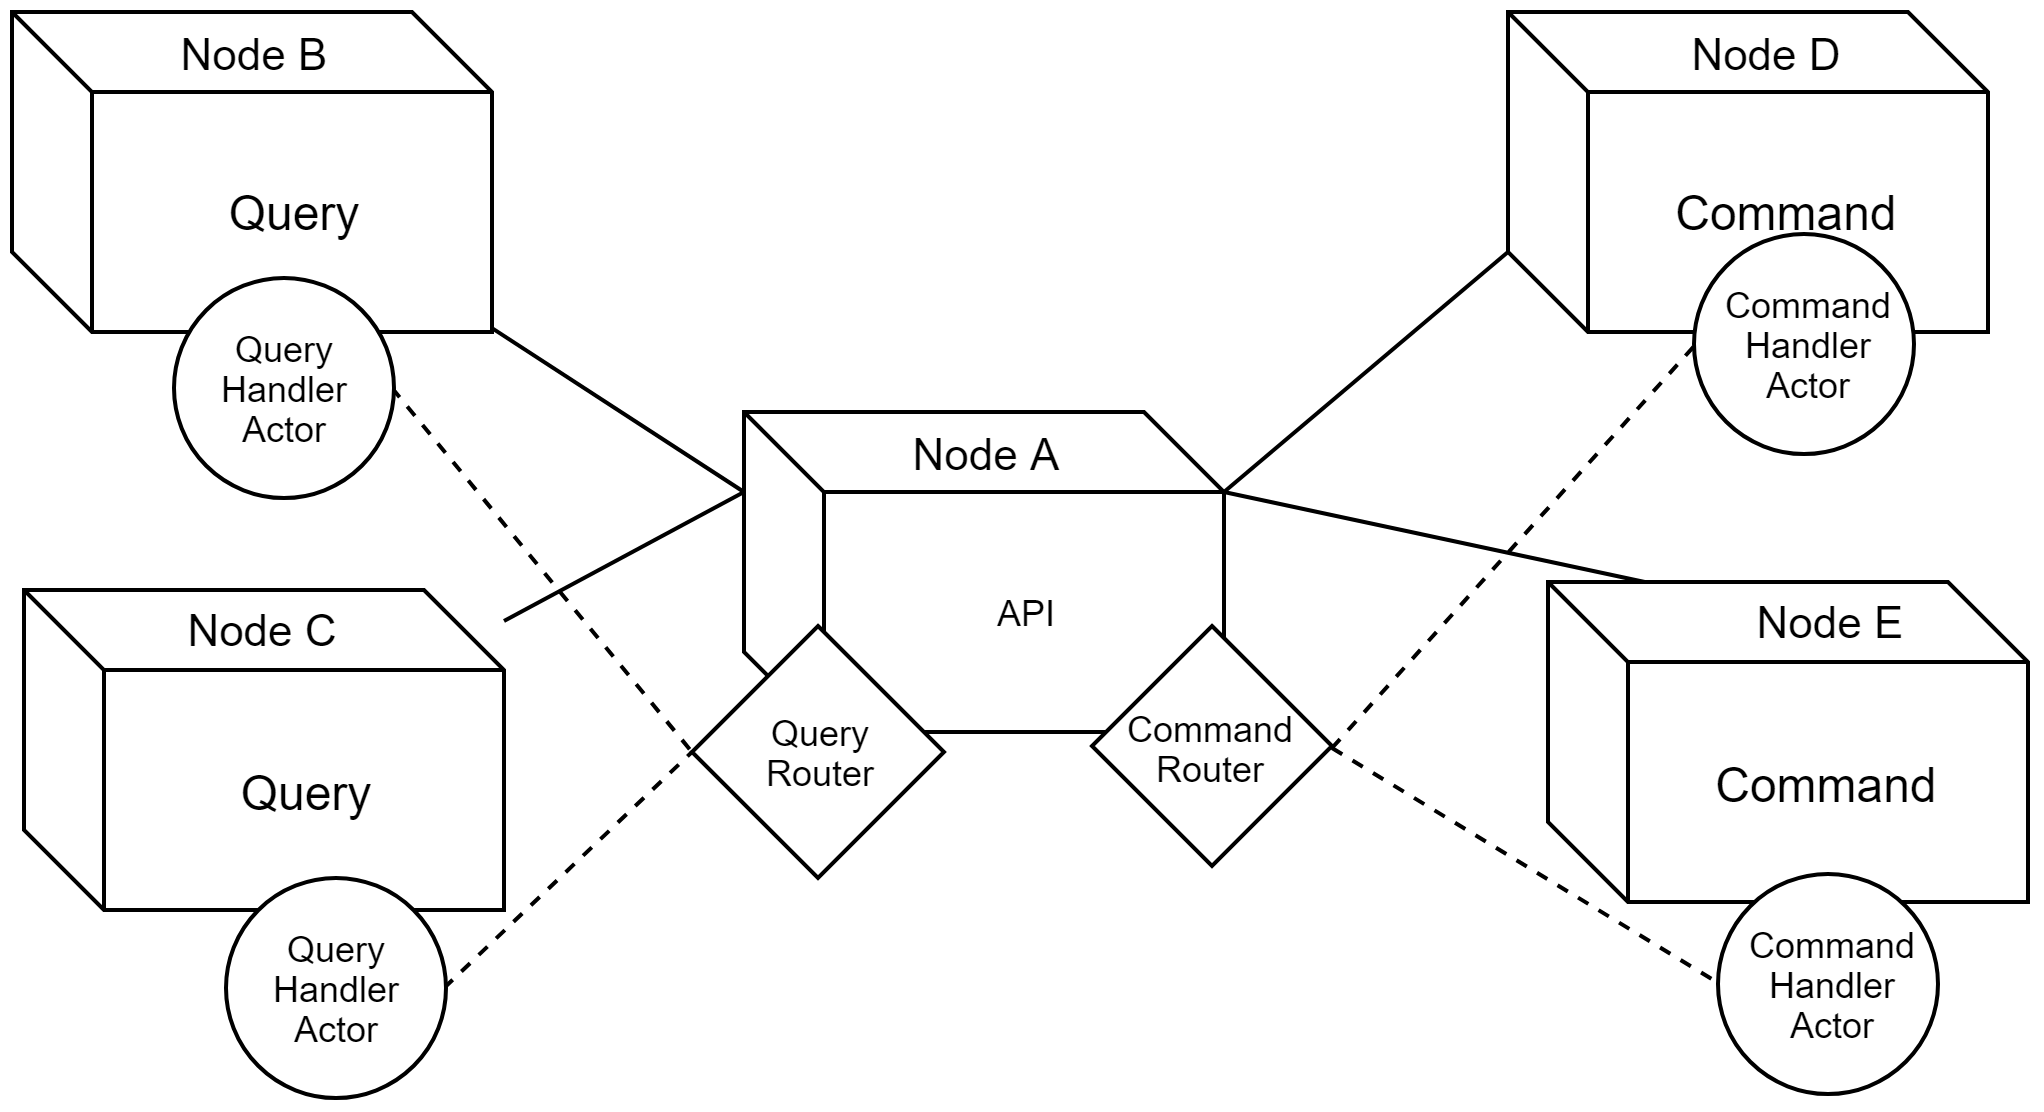
\includegraphics[width=\linewidth]{gfx/implementation/ClusterRouter}
    \caption{Ein verteiler \textit{Round-Robin} Router welcher Nachrichten von der Komponente \textit{API} auf andere Komponenten verteilt.}
    \label{fig:implementation:routing}
\end{figure} 



\subsection{Gossip}
\label{subsec:implementation:gossip}
Bereits in Abschnitt \ref{subsec:implementation:lighthouse} wurde die Komponente \textit{Lighthouse} vorgestellt, welche als Einstiegspunkt für alle Nodes verwendet wird. Die Verbindung zu den restlichen im Cluster vorhandenen Nodes, wird über das \textit{Gossip} Protokoll hergestellt. \\
Der Name \textit{Gossip} leitet sich vom Geschwätz mehrerer Personen ab, jeder erzählt einem anderen etwas, und so wissen alle über jeden anderen  bescheid. Das gleiche Prinzip wird in diesem Protokoll verwendet, um Änderungen an einem einzelnen Node allen anderen Nodes im Cluster bekannt zu geben. \\
Nodes mit der Rolle \textit{Lighthouse} sind der Start dieser Kommunikation. Deshalb müssen diese Nodes auch über eine fixe Adresse verfügen, im Fall von \textit{TyrolSky} sind das Ip-Addresse und Port. Komponenten welche nun dem Cluster beitreten wollen, melden sich bei einem der \textit{Lighthouse} Komponenten an, und geben bekannt über welche Adresse sie erreichbar sind. Über das \textit{Gossip} Protokoll wird nun jedem bereits im System beigetretenen Node mitgeteilt das sich ein neuer Node im Cluster befindet. \\
In der Kommunikation zwischen den Nodes wird den anderen Nodes auch mitgeteilt, welche Rollen eine Komponenten besitzt. Dies wird dann anschließend von den Routern, siehe Abschnitt \ref{fig:implementation:routing}, verwendet, um Nachrichten an die diese Rollen zuzustellen. Weiters beinhaltet das Protokoll auch Informationen über den Zustand der einzelnen Nodes. Bei einer fehlerhaften Verbindung zwischen zwei Nodes werden alle anderen Nodes über den Fehlerzustand benachrichtigt. Ist ein Node nicht mehr erreichbar ohne das eine kontrollierte abmeldung vom Cluster stattgefunden hat, kann er jedoch nicht einfach aus dem Cluster entfernt werden sondern es muss eine Lösungsstrategie implementiert sein, siehe dazu den nachfolgenden Abschnitt \ref{subsec:implementation:splitBrain}. \\ 
Das Protokoll dient neben der Zusammenfügung der einzelnen Node zu einem Cluster auch zum austausch von Informationen über den aktuellen Zustand des Clusters. Muss vom Protokoll eine entscheidung getroffen werde, wie beispielsweiße die Entscheidung über den Beitritt zum Cluster, wird ein Node ausgewählt, welcher die Führung über den Cluster übernimmt. Im Fall von \textit{TyrolSky} ist das immer der ältester Node im Cluster, wird dieser vom Cluster entfernt, übernimmt die Führung der nächst älteste Node.  

\subsection{Split Brain} 
\label{subsec:implementation:splitBrain}

\subsection{Globale Dienste}
\label{subsec:implementation:singeltons}

\subsection{Verteilung transaktionaler Daten}
\label{subsec:implementation:akkaSharding}
Erklärung von Sharding
